\documentclass[pdf,color]{UoBnote}
\usepackage{epstopdf}
\author{Samuel Delacruz\\
				sjd054@bham.ac.uk\\
				1090154}

\shorttitle{Worksheet 2}
\title{Computational Modelling of Physical Systems\\Worksheet 2}
\date{\today}
\issue{2}

\begin{document}

\maketitle
\tableofcontents
\vspace{1cm}\hrule \vspace{1cm}
%\newpage

\section{Introduction}
\section{Numerical Integration}
	\subsection{The Trapezium Rule}
		\subsubsection{Theory}
			The trapezium rule can be used as a method of numerically evaluating integrals. It involves splitting a function $f(x)$ into $n$ intervals of separation $h$,
			connected by straight lines. These pieces can be integrated by creating trapzoidal segments and calculating their area, then summing their areas.
			and using their area to approximate the integral of $f(x)$. As $h \rightarrow 0$, the estimated value converges to the exact integral value. The trapezium rule is given as follows:
			
			\begin{equation} \label{eq:trapezium}
				\int\limits_{x_0}^{x_n} f(x) dx \approx \frac{1}{2}h\left[f(x_0) + f(x_n) + 2(f(x_1) + f(x_2) +...+ f(x_{n-1}))\right]
			\end{equation}
			
			Where $h$, the width of the interval is defined by:
			
			\begin{equation} \label{eq:h_def}
				h = \frac{x_n - x_0}{n}
			\end{equation}
			
			Due to the nature of the trapezium rule, there is naturally an error associated with values calculated using it.
			There exists an analytic expression for this error and is given by the following equation $^{\cite{errors_web}}$:
			
			
			\begin{equation} \label{eq:trap_err}
				E_n^T = -\frac{h^2\left(b-a\right)}{12}f''(c_n)
			\end{equation}
			
			Which can be adapted to give the maximum error on the estimated value for the integral of $f(x)$:
			
			\begin{equation} \label{eq:trap_err2}
				\left|E_n^T\right| \leq \frac{h^2\left(b-a\right)}{12}\max_{a \leq x \leq b}\left|f''(x)\right|
			\end{equation}
			
			\subsubsection{Procedure}
				
				\begin{figure}[tb]
					\centering
						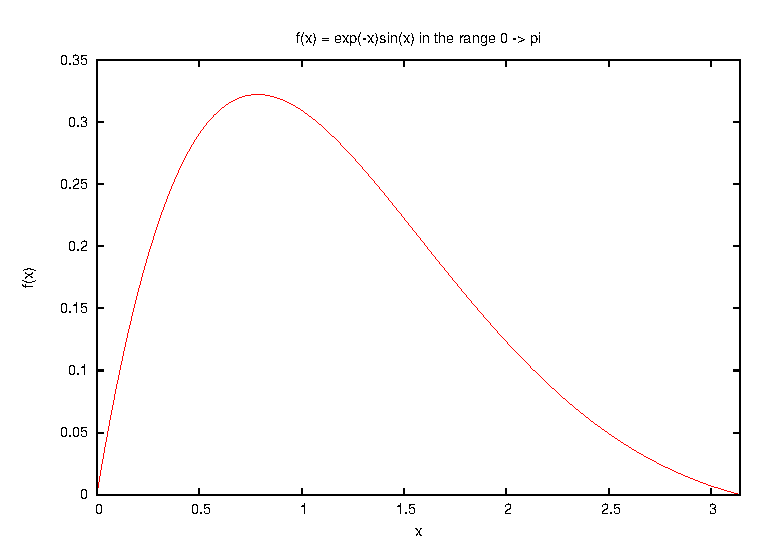
\includegraphics{figures/q2b.eps}
					\caption{Plot of $f(x)$ in the range $[0:\pi]$}
					\label{fig:q2b}
				\end{figure}
				
				
				\begin{figure}[tb]
					\centering
						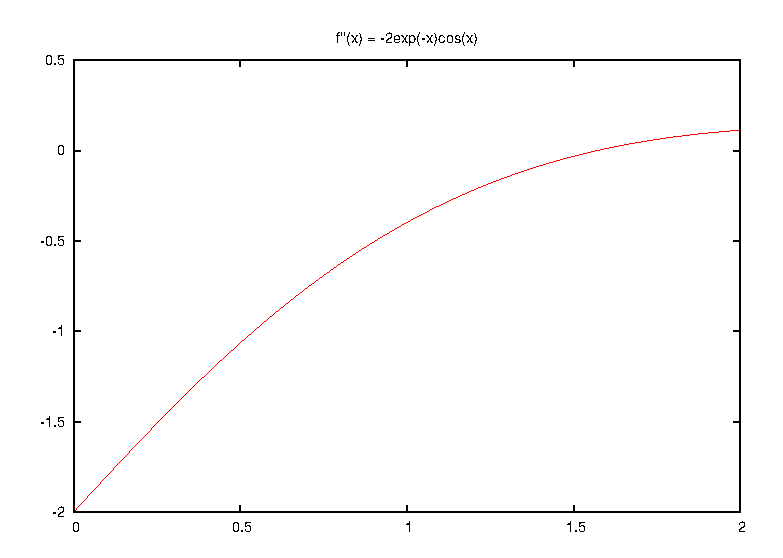
\includegraphics{figures/q2-f2x-trap.eps}
					\caption{Plot of $f''(x)$ in the range $[0:2]$}
					\label{fig:q2-f2x-trap}
				\end{figure}
				
				
			
		\subsection{Simpson's Rule}
			\subsubsection{Theory}
				Simpson's rule is another method of computing the value of integrals. Instead of splitting $f(x)$ into straight-line segments as in the trapezium rule, the function is split into a
				series of parabolic segments. This results in a higher level of precision than the trapezium rule, and will be demonstrated in the procedure to follow. The equation for Simpson's rule is given as follows $^{\cite{errors_web}}$:
				
				\begin{equation} \label{simpsons}
					\int\limits_a^b f(x) dx \approx \frac{h}{3}\left[f(x_0) + 4f(x_1) + 2f(x_2) + 4f(x_3) + 2f(x_4) + ... + 2f(x_{n-2}) + 4f(x_{n-1}) +f(x_n)\right]
				\end{equation}
				
				Which may also be written as $^{\cite{simps_wiki}}$:
				
				
				\begin{equation} \label{simpsons_sum}
					\int\limits_a^b f(x) dx \approx \frac{h}{3}\left[f(x_0) + 2 \sum\limits_{j=1}^{(n/2)-1} \left(f(x_{2j})\right) + 4 \sum\limits_{j=1}^{n/2} \left(f(x_{2j-1})\right) + f(x_n) \right]
				\end{equation}
				Where $h$ is given in equation (\ref{eq:h_def})
				
			\subsubsection{Procedure}
				
				\begin{figure}[tb]
					\centering
						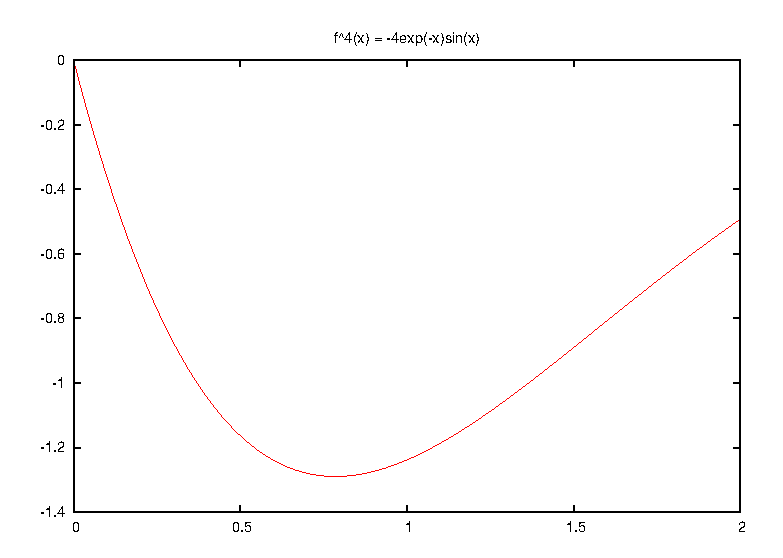
\includegraphics{figures/q2-f4x-simps.eps}
					\caption{Plot of $f^{\left(4\right)}(x)$ in the range $[0:2]$}
					\label{fig:q2-f4x-simps}
				\end{figure}
				
				
\section{Numerical Integration with GSL}

\section{Appendices}

\begin{thebibliography}{breitestes Label}
	\bibitem{errors_web} Kendall E. Atkinson\\{\em http://homepage.math.uiowa.edu/\textasciitilde{}atkinson/ftp/ENA\_Materials/Overheads/sec\_5-2.pdf}\\Accessed at 01-11-2013\\
	\bibitem{simps_wiki} Wikipedia.org\\{\em http://en.wikipedia.org/wiki/Simpson's\_rule\#Composite\_Simpson.27s\_rule}\\Accessed at 01-11-2013
\end{thebibliography}

\end{document}
